\section{Methodology}
\label{section:methodology}

% In this section we describe the methodology of our research

En la Figura \ref{figure:awesome_figure} podemos observar que es una gráfica muy bonita.

\lipsum[1]

% Example of illustrative figure
\begin{figure}[htb]
  \caption{The title of our enlightening figure}
  \label{figure:awesome_figure}
  \centering 
  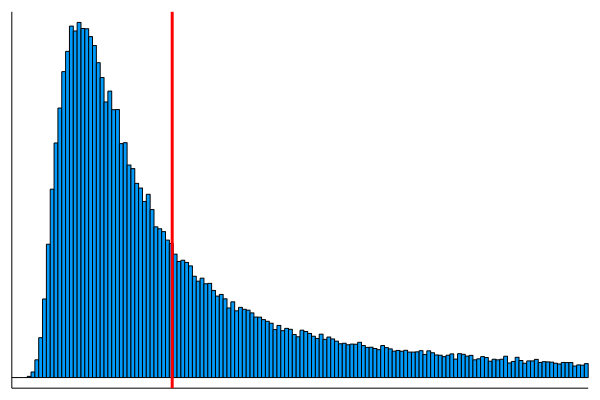
\includegraphics[width=0.9\textwidth]{figures/mse_distribution.png}
  \caption*{\footnotesize Note: error is computed as the standard deviation of the set of realizations... .}
\end{figure}

\lipsum[1]

Here goes a snippet of code in \ref{lst:mylabel}... 

\lstinputlisting[caption={My very special computer code}, label={lst:mylabel}]{code/testfile.jl}

In snippet \ref{lst:small_snippet} we observe... 

\begin{lstlisting}[caption={A small snippet}, label={lst:small_snippet}]
function myfn(a,b,kw...)
  g = 2a - b
end
\end{lstlisting}